\documentclass{standalone}
\usepackage{tikz}
\begin{document}
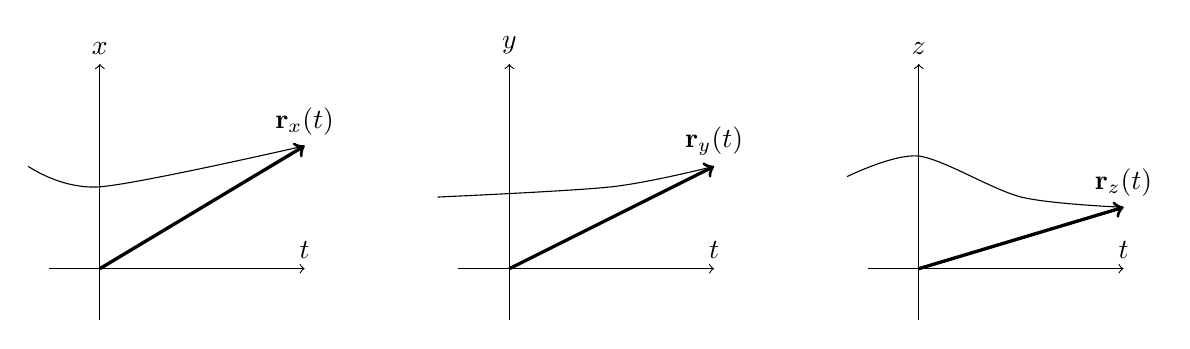
\begin{tikzpicture}[scale=1.3]
    \coordinate (O) at (-4,0);
    \draw[->] (-4.5, 0) -- (-2, 0) coordinate (t) node[above]{$t$};
    \draw[->] (-4,-0.5) --(-4,2) coordinate (x) node[above]{$x$};
    \draw[->,very thick] (O) -- (-2, 1.2) node[above] {$\mathbf{r}_x(t)$};
    \draw[-]plot[smooth]coordinates{(-4.7,1)(-4,0.8)(-2, 1.2)};


    \coordinate (O) at (0,0);
    \draw[->] (-0.5, 0) -- (2, 0) coordinate (t) node[above]{$t$};
    \draw[->] (0,-0.5) --(0,2) coordinate (y) node[above]{$y$};
    \draw[->,very thick] (O) -- (2, 1) node[above] {$\mathbf{r}_y(t)$};
    \draw[-]plot[smooth]coordinates{(-0.7,0.7)(1,0.8)(2, 1)};

    \coordinate (O) at (4,0);
    \draw[->] (3.5, 0) -- (6, 0) coordinate (t) node[above]{$t$};
    \draw[->] (4,-0.5) --(4,2) coordinate (z) node[above]{$z$};
    \draw[->,very thick] (O) -- (6, 0.6) node[above] {$\mathbf{r}_z(t)$};
    \draw[-]plot[smooth]coordinates{(3.3,0.9)(4,1.1)(5,0.7)(6, 0.6)};

\end{tikzpicture}
\end{document}